%! alt Triangle ABC with BC = 20, CA = 15 and AB = 7, its incircle with centre I and radius 2, and the dashed inner triangle A'B'C', the image of ABC under the homothety at I with ratio 1/2. The coin of radius 1 is drawn pushed into each corner, centred at the vertices A', B' and C' of the inner triangle. At each vertex of ABC the shaded kite has corners at the vertex, the two points where the coin touches the sides, and the coin's centre; the part of the kite outside the coin is never covered. Dashed segments join I to C and to the incircle's points of contact on BC and CA, outlining the incircle's kite at C, which is twice the size of the coin's kite at C.
%! after_paragraph 3
%! scale 21/50
% The shared preamble of every Cevian figure. pipeline/figures turns these colours into theme-aware paint,
% and refuses any other colour, so draw only with them:
%   figink (lines and labels), figaux (construction lines), figaccent (the object the argument turns on),
%   figtint and figaccenttint (light fills).
\documentclass[border=1.5pt]{standalone}
\usepackage{tkz-euclide}
\definecolor{figink}{RGB}{0,0,0}
\definecolor{figaux}{RGB}{85,85,85}
\definecolor{figaccent}{RGB}{192,57,43}
\definecolor{figtint}{RGB}{221,221,221}
\definecolor{figaccenttint}{RGB}{245,213,208}
% tkz-euclide's defaults draw circles, compasses and marks in 50% grey and fill points with a tint.
\makeatletter
\def\tkz@otherlinecolor{figink}
\def\tkz@euc@circlecolor{figink}
\def\tkz@euc@compasscolor{figink}
\def\tkz@euc@mkcolor{figink}
\def\tkz@mk@fill{figink}
\def\tkz@euc@pointfillcolor{figink}
\makeatother
\tkzSetUpLine[color=figink,line width=.7pt]
\tkzSetUpArc[color=figink,line width=.7pt]
\tkzSetUpCompass[color=figink,line width=.5pt]
\tkzSetUpPoint[color=figink,fill=figink,size=3.1pt]
\tikzset{
  every picture/.style={line cap=round,line join=round,color=figink},
  circle style/.append style={color=figink,line width=.7pt},
  aux/.style={color=figaux,line width=.45pt,dash pattern=on 2.6pt off 2pt},
  key/.style={color=figaccent,line width=1pt},
  mk/.style={color=figink,line width=.5pt},
  lbl/.style={color=figink,inner sep=2.2pt},
  len/.style={color=figink,inner sep=1.5pt,font=\small},
}

\begin{document}
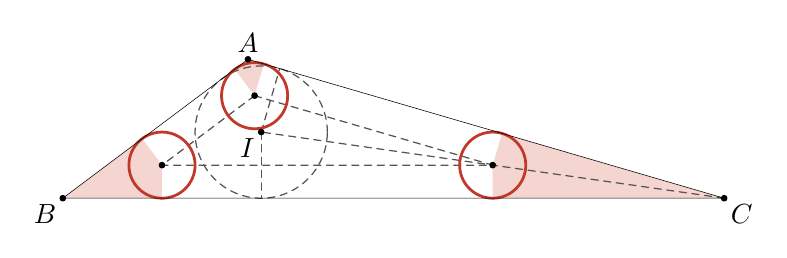
\begin{tikzpicture}
\tkzDefPoint(0.0,0.0){B} %! B = (0, 0)
\tkzDefPoint(8.4000000,0.0){C} %! C = (20, 0)
\tkzDefPoint(2.3520000,1.7640000){A} %! A = (28/5, 21/5)
\tkzDefPoint(2.5200000,0.84000000){I} %! I = incentre(A, B, C)
\tkzDefPoint(2.4360000,1.3020000){Ap} %! Ap = lerp(I, A, 1/2)
\tkzDefPoint(1.2600000,0.42000000){Bp} %! Bp = lerp(I, B, 1/2)
\tkzDefPoint(5.4600000,0.42000000){Cp} %! Cp = lerp(I, C, 1/2)
\tkzDefPoint(2.1840000,1.6380000){Xa} %! Xa = foot(Ap, A, B)
\tkzDefPoint(2.5536000,1.7052000){Ya} %! Ya = foot(Ap, A, C)
\tkzDefPoint(1.2600000,0.0){Xb} %! Xb = foot(Bp, B, C)
\tkzDefPoint(1.0080000,0.75600000){Yb} %! Yb = foot(Bp, B, A)
\tkzDefPoint(5.4600000,0.0){Xc} %! Xc = foot(Cp, C, B)
\tkzDefPoint(5.5776000,0.82320000){Yc} %! Yc = foot(Cp, C, A)
\tkzDefPoint(2.5200000,0.0){D} %! D = foot(I, B, C)
\tkzDefPoint(2.7552000,1.6464000){E} %! E = foot(I, C, A)
%! fact dist(B, C) == 20
%! fact dist(C, A) == 15
%! fact dist(A, B) == 7
%! fact area(A, B, C) == 42
%! fact inradius(A, B, C) == 2
%! fact dist(I, D) == 2
%! fact dist(I, E) == 2
%! fact tangent(Ap, 1, A, B)
%! fact tangent(Ap, 1, A, C)
%! fact tangent(Bp, 1, B, C)
%! fact tangent(Bp, 1, B, A)
%! fact tangent(Cp, 1, C, B)
%! fact tangent(Cp, 1, C, A)
%! fact tangent(I, 2, B, C)
%! fact parallel(Ap, Bp, A, B)
%! fact parallel(Bp, Cp, B, C)
%! fact parallel(Cp, Ap, C, A)
%! fact collinear(Cp, C, I)
%! fact midpoint(Xc, C, D)
%! fact midpoint(Yc, C, E)
%! fact area(A, Xa, Ap, Ya) + area(B, Xb, Bp, Yb) + area(C, Xc, Cp, Yc) == 21/2
%! fact area(Ap, Bp, Cp) == 21/2
%! fact dist(Ap, Bp) + dist(Bp, Cp) + dist(Cp, Ap) == 21
%! example dist(C, Xc) == 7
%! example dist(B, Xb) == 3
%! example dist(A, Xa) == 1/2
\tkzFillPolygon[color=figaccenttint](A,Xa,Ap,Ya)
\tkzFillPolygon[color=figaccenttint](B,Xb,Bp,Yb)
\tkzFillPolygon[color=figaccenttint](C,Xc,Cp,Yc)
\tkzDrawCircle[aux](I,D)
\tkzDrawPolygon[aux](Ap,Bp,Cp)
\tkzDrawSegments[aux](I,D I,E C,I)
\tkzDrawCircle[key](Ap,Xa)
\tkzDrawCircle[key](Bp,Xb)
\tkzDrawCircle[key](Cp,Xc)
\tkzDrawPolygon(A,B,C)
\tkzDrawPoints(A,B,C,I,Ap,Bp,Cp)
\tkzLabelPoint[above,lbl](A){$A$}
\tkzLabelPoint[below left,lbl](B){$B$}
\tkzLabelPoint[below right,lbl](C){$C$}
\tkzLabelPoint[below left,lbl](I){$I$}
\end{tikzpicture}
\end{document}
